%!TEX root = ../scivis_lbaakman_bvanloon.tex
This section discusses the color maps provided in the application. Each color map is accompanied with a short discussion of its advantages, disadvantages and in which situations it is best applied. 

As discussed in the previous section, color maps provide a way to map scalar values to colors in order for the user to extract information. The quality of a color map can be judged by how well and intuitive the color map allows inverse mapping. Which color map is best depends on the context and the goal of the visualization. For example the zebra color map is well suited to the visualization of scalar values that vary quickly, \ie the first derivative, but is less useful if the aim was to highlight maximum values. Historical reasons can also influence the choice of color maps. For example X-rays are for example always displayed with a gray-scale color map, in spite of the existence of alternative color maps.

In our application we have chosen to implement a variety of color maps, this way the application offers a suitable color map for almost any form of visualization, ranging from the (in)famous rainbow color map to luminance based, two-hue and diverging color maps.

\begin{figure}[b]
	\begin{subfigure}{1\textwidth}
		\begin{minipage}[l]{0.05\textwidth}
	    	\caption{} \label{fig:colormaps:legends:rainbow}
	  	\end{minipage}
	  \hfill
	  	\begin{minipage}[l]{0.95\textwidth}
	    	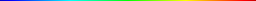
\includegraphics[width=\textwidth,height=15px,keepaspectratio=false,frame]{colormapping/img/colormap_legends/rainbowcolormap.png}
	  	\end{minipage}
	\end{subfigure}

  	\begin{subfigure}{1\textwidth}
  		\begin{minipage}[l]{0.05\textwidth}
    		\caption{} \label{fig:colormaps:legends::zebra}
  		\end{minipage}
  	\hfill
  		\begin{minipage}[l]{0.95\textwidth}
    		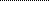
\includegraphics[width=\textwidth,height=15px,keepaspectratio=false,frame]{colormapping/img/colormap_legends/zebracolormap.png}
  		\end{minipage}
  	\end{subfigure}

  	\begin{subfigure}{1\textwidth}
  		\begin{minipage}[l]{0.05\textwidth}
    		\caption{} \label{fig:colormaps:legends::grayscale}
  		\end{minipage}
  	\hfill
  		\begin{minipage}[l]{0.95\textwidth}
    		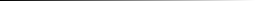
\includegraphics[width=\textwidth,height=15px,keepaspectratio=false,frame]{colormapping/img/colormap_legends/grayscalecolormap.png}
  		\end{minipage}
  	\end{subfigure}
  	\begin{subfigure}{1\textwidth}
  		\begin{minipage}[l]{0.05\textwidth}
    		\caption{} \label{fig:colormaps:legends::heat}
  		\end{minipage}
  	\hfill
  		\begin{minipage}[l]{0.95\textwidth}
    		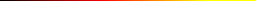
\includegraphics[width=\textwidth,height=15px,keepaspectratio=false,frame]{colormapping/img/colormap_legends/heatcolormap.png}
  		\end{minipage}
  	\end{subfigure}
  	\begin{subfigure}{1\textwidth}
  		\begin{minipage}[l]{0.05\textwidth}
    		\caption{} \label{fig:colormaps:legends::cold}
  		\end{minipage}
  	\hfill
  		\begin{minipage}[l]{0.95\textwidth}
    		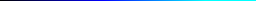
\includegraphics[width=\textwidth,height=15px,keepaspectratio=false,frame]{colormapping/img/colormap_legends/coldcolormap.png}
  		\end{minipage}
  	\end{subfigure}
  	\begin{subfigure}{1\textwidth}
  		\begin{minipage}[l]{0.05\textwidth}
    		\caption{} \label{fig:colormaps:legends::hue}
  		\end{minipage}
  	\hfill
  		\begin{minipage}[l]{0.95\textwidth}
    		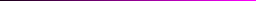
\includegraphics[width=\textwidth,height=15px,keepaspectratio=false,frame]{colormapping/img/colormap_legends/huecolormap.png}
  		\end{minipage}
  	\end{subfigure}
  	\begin{subfigure}{1\textwidth}
  		\begin{minipage}[l]{0.05\textwidth}
    		\caption{} \label{fig:colormaps:legends::twocolors}
  		\end{minipage}
  	\hfill
  		\begin{minipage}[l]{0.95\textwidth}
    		
\includegraphics[width=\textwidth,height=15px,keepaspectratio=false,frame]{colormapping/img/colormap_legends/twocolorscolormap.png}
  		\end{minipage}
  	\end{subfigure}
  	\begin{subfigure}{1\textwidth}
  		\begin{minipage}[l]{0.05\textwidth}
    		\caption{} \label{fig:colormaps:legends::diverging}
  		\end{minipage}
  	\hfill
  		\begin{minipage}[l]{0.95\textwidth}
    		
\includegraphics[width=\textwidth,height=15px,keepaspectratio=false,frame]{colormapping/img/colormap_legends/divergingcolormap.png}
  		\end{minipage}
  	\end{subfigure}
\caption{Color maps provided in the application: 
(\subref{fig:colormaps:legends:rainbow}) rainbow, 
\subref{fig:colormaps:legends::zebra} zebra,
\subref{fig:colormaps:legends::grayscale} gray-scale,
\subref{fig:colormaps:legends::heat} heat,
\subref{fig:colormaps:legends::cold} cold,
\subref{fig:colormaps:legends::hue} user picked hue,
\subref{fig:colormaps:legends::twocolors} linear two-color, and
\subref{fig:colormaps:legends::diverging} blue-red diverging. Each color map is shown using full saturation and 256 colors, except for the zebra color map which has 50 `colors'. }
\label{fig:colormaps:legends}
\end{figure}


\subsection{Rainbow Colormap} % (fold)
\label{ssub:rainbow_colormap}
The rainbow color map, illustrated in \cref{fig:colormaps:legends:rainbow} is one of the most used color maps in the scientific community and is therefore included in our application. The color map is constructed by first doing a piecewise interpolation of blue to green and next from green to red. The resulting colors are a mix of blue and green or a mix of green and red, except for the tails of the color map which contain only blue or red.

The color map is often seen as visually appealing due to the varying colors and can give an intuitively mapping of high and low values to warm (red) and cold (blue) colors. However, although often used, the rainbow color map has many flaws and is heavily critiqued\cite{borland2007rainbow,divergingMoreland2009}. Some of the main disadvantages of this color map are discussed below.
\begin{itemize}
  \item It pulls the focus of its users towards areas with high values. This can be an advantage when these are the values of interest, but it might distract otherwise.
  \item All colors in the color map have the same luminance, except for its most extreme colors, but many perceive the colors in this color map to have different luminosity. As a result the ordering of the luminance in the colormap might appear to be non-monotonic, which can confuse the inverse mapping process.
  \item There is no decisive ordering of the colors in this color map. It orders the colors from blue, to green, to yellow, to red, which is not a order naturally perceived.
  \item The color map does not behave well when the saturation is lowered or when translated to black and white, for example when printing in black and white. Doing so results in a broken, non-monotonic color map, which disallows proper inverse mapping.
  \item It is not is not colorblind friendly.
\end{itemize}

% subsubsection flaws (end)


\subsection{Luminance Color maps} % (fold)
\label{sub:luminance_colormaps}
The next set of color maps use luminance to give a natural ordering of the colors (and thus values). These color maps are often effective since human perception is sensitive to changes in luminance\cite{divergingMoreland2009} which makes inverse mapping easier. Luminance based color maps have three major disadvantages. Firstly they are not well-suited for use in combination with 3D shading, since shading can cause changes in the perceived luminance of a color or vice verse changes in luminance might give the illusion of shading, where there is none. Secondly luminance based color maps draw attention to areas with high luminance, details in low luminosity areas are often hard to see and are therefore likely to be overlooked. A third flaw is that pixels with the same luminance might look different depending on the luminance of the surrounding pixels. We support for different luminance color maps, which are discussed in \crefrange{ssub:gray_scale_colormap}{ssub:cold_colormap}.
% subsection luminance_colormaps (end)

\subsubsection{Gray-Scale color map} % (fold)
\label{ssub:gray_scale_colormap}
The gray-scale color map is given shown \cref{fig:colormaps:legends::grayscale} is the simplest of the luminance based color maps and does not use any hue. The advantage of this color map is that it works well for a lot of media and does not rely on changes in hues for inverse mapping. This makes this color map suitable for many applications and users. Besides the general disadvantages associated with luminance based color maps, this specific color map is not well suited to non compact datasets, e.g. datasets containing holes. In these cases the background might be similar to objects in the dataset, making them blend into the background.


\subsubsection{Single Hue Color map} % (fold)
\label{ssub:single_hue_colormap}
The single hue color map is an extension on the gray-scale color map. This color map is created by adding a single hue to the gray-scale color map. This can make the color map more visual appealing and removes the probability of the visualization blending in with the background. In \cref{fig:colormaps:legends::hue} an example is shown, using a pink hue.

\subsubsection{Heat Colormap} % (fold)
\label{sub:heat__colormap}
The heat map is a luminance based color map that uses both luminance and a range of hues for the ordering and thus provides more clues as to the ordering of the colors, compared to the gray-scale and single hue color map. Although it uses less hues than the rainbow color map it has as the advantage that the used hues have a natural perceived ordering, namely red, to orange, to yellow.

In some applications the heat color map uses white for the highest value data instead of the yellow we use. Since our application has a white background, we removed the white value from the color map. The color map is displayed in \cref{fig:colormaps:legends::heat}.


\subsubsection{Cold Color map} % (fold)
\label{ssub:cold_colormap}
The cold color map is similar to the heat color map except it uses blue tinted colors instead of red tints. It is added since blue and red are nice contrasting colors making it possible to combine scalar visualization with glyphs by using the heat map for one visualization and the cold color map for the second visualization. The color map is displayed in \cref{fig:colormaps:legends::cold}.

\subsection{Isoluminant Color map} % (fold)
\label{sub:two_hue_colormap}
The isoluminant color map, shown in \cref{fig:colormaps:legends::twocolors}, is a cyan-to-mauve color map based on linear interpolation\cite{divergingMoreland2009}. Because the color map is isoluminant it is well suited to be used in combination with 3D shading since differences in luminance can only be caused by shading. Opposed to the green-to-red isoluminant color map that is also often used, the cyan-to-mauve color map is colorblind friendly, making it a more suitable candidate. Although well suited for use in 3D visualizations the color map has two major flaws. The human perception is less sensitive to changes in hue than in changes in luminance, making the inverse mapping processes of this color map harder than it is for luminance based color maps. Furthermore, since the color map offers less color variation than a lot of other color maps it is  difficult to visualize a large range of values, the colors of the resulting visualization are often perceived as dull.
% subsection two_hue_colormap (end)

\subsection{Diverging Color map} % (fold)
\label{sub:diverging_colormap}
The diverging color map is constructed by the interpolation of two hues at the end of the color map with a middle hue. In other words, given three colors $c_{\text{min}}$, $c_{\text{mid}}$, and $c_{\text{max}}$ the color map is constructed by first interpolating $c_{\text{min}}$ and $c_{\text{mid}}$ and next interpolating $c_{\text{mid}}$ and $c_{\text{max}}$. In our application the three colors are taken from \cite{divergingMoreland2009}, which proposes a blue tint for $c_{\text{min}}$, an off-white for $c_{\text{mid}}$ and a red tint for $c_{\text{max}}$. The resulting color map is shown in \cref{fig:colormaps:legends::diverging}. 

The diverging color map is mostly used in cases the median value is of importance. By the interpolating three colors the areas where the scalars approximate the median value are clearly distinguishable by their white color. Furthermore there is a clear separation between scalars greater than and smaller than the median value, the first are shown in red, the second in blue. A disadvantage of the diverging color map is that there is no clear natural ordering of the colors. Furthermore separation of the scalars by their median value is not always relevant.

\subsection{Zebra Color map} % (fold)
\label{sub:zebra_colormap}
The zebra color map differs significantly from the previously discussed color maps. It only uses two alternating colors and thus does not offer an inverse mapping from color to scalar value. However, the color map is very useful for showing variations in the data. It can be used to detect regions in which data changes quickly or alternatively, where data stays constant. When applying the color map to the data, care should be taken that the number of colors is not too high. When this is the case the black/white bands might vary too quickly and blend together into a gray area and thus results in false colors. \cref{fig:colormaps:legends::zebra} gives an example of the color map, with 50 color bands.